\chapter{Vyhodnocení}
\section{Vyhodnocení sběru dat a spolehlivosti} \label{sec:resData}
    Pro účely této práce se sbírala data (\cref{chap:dataCollection}) od \DTMdisplaydate{2021}{12}{09}{-1} \DTMdisplaytime{17}{38}{00} (UTC) do \DTMdisplaydate{2022}{05}{02}{-1} \DTMdisplaytime{11}{59}{00} (UTC). Za tu dobu bylo sesbíráno 38128~vzor\-ků dat, sestávajících z 15 hodnot příznakových veličin, 2 hodnot stavu žaluzie, časové známky, důvodu pořízení vzorku a aktivity testovacího režimu. Z toho bylo 36306 pořízeno periodicky v pětiminutových intervalech a 1822 na základě události změny stavu žaluzie - ruční ovládání uživatelem. Příklad 3 sbíraných veličin na časovém úseku jednoho dne (\DTMdisplaydate{2022}{04}{19}{-1}) je v grafu na \refskl{fig:data_sel}{obrázku}.
    \begin{figure}[H]
        \centering
        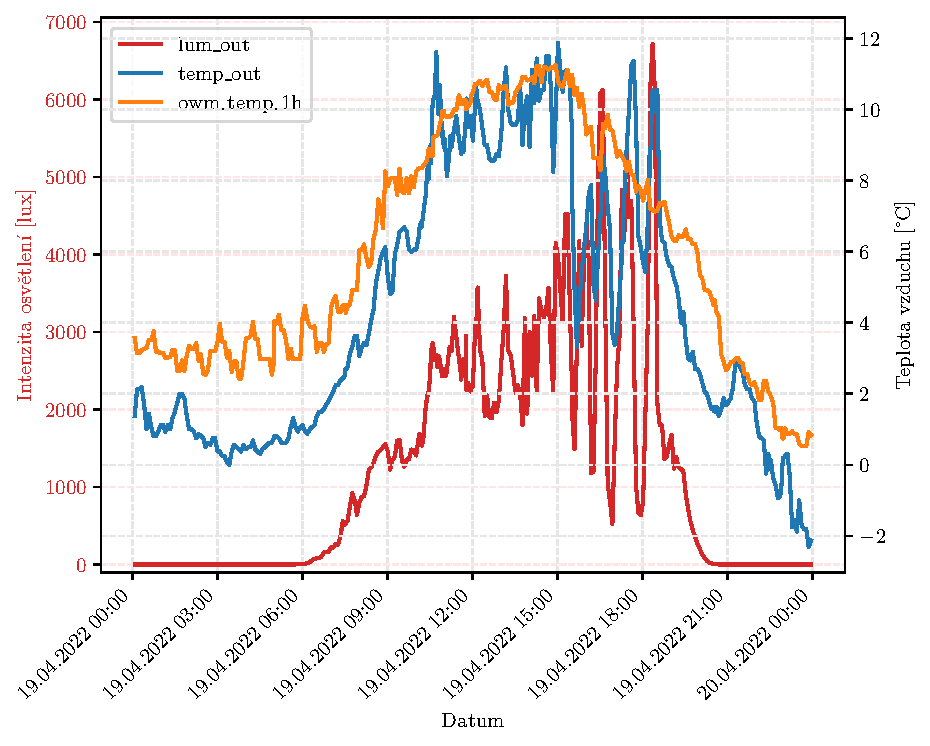
\includegraphics[draft=false,width=\textwidth]{img/results/data_sel.pdf}
        \caption[Graf sesbíraných dat (příklad)]{Graf sesbíraných hodnot 3 vybraných příznakových veličin z celkových 15. Zobrazena je pouze část dat ze dne \DTMdisplaydate{2022}{04}{19}{-1}}
        \label{fig:data_sel}
    \end{figure}

    V průběhu sběru dat došlo ke 125~výpadkům při kterých bylo ztraceno 5240~vzorků. Nejčastějším důvodem výpadku byly problémy s připojením k \acrshort{api} výrobce žaluzie (Somfy, celkem 105 výpadků). Mezi další příčiny patří výpadky senzorů (odpojení), plný disk databázového serveru (MongoDB) a chyba v systému domácí automatizace (Home Assistant). Poslední dvě příčiny společně způsobily ztrátu asi 81~\% měření z celkového počtu ztracených měření. Největší z výpadků, způsobený Home Assistantem, vznikl ještě před implementací monitoringu přicházejích MQTT zpráv a byl tak odhalen pozdě. Jednou došlo k výpadku připojení k DNS serverům poskytovatele připojení k internetu a nebylo kvůli tomu možné zjistit stav žaluzie. Počet výpadků, jejich důvod a počet při nich ztracených měření shrnuje \cref{tab:outages}.
    % Table generated by Excel2LaTeX from sheet 'List1'
\begin{table}[htbp]
  \centering
  \begin{tabular}{l|r|r}
    \toprule
    Důvod výpadku & \multicolumn{1}{l|}{Počet výpadků} & \multicolumn{1}{l}{Počet ztracených vzorků} \\
    \midrule
    \midrule
    Somfy & 105   & 383 \\
    \midrule
    Senzory & 14    & 605 \\
    \midrule
    MongoDB & 4     & 2244 \\
    \midrule
    DNS   & 1     & 27 \\
    \midrule
    Home Assistant & 1     & 1981 \\
    \midrule
    Celkem & 125   & 5240 \\
    \bottomrule
    \bottomrule
    \end{tabular}%
  \caption[Výpadky]{Výpadky součástí systému automatického ovládání žaluzií při sběru dat a výpadky třetích stran, na kterých je systém závislý.}
  \label{tab:outages}%
\end{table}%


    Vzorky podle důvodu sběru (událost, periodické) a výpadky v závislosti na čase jsou v grafu na \refskl{fig:sample_type}{obrázku}. Každý vzorek je vyobrazen jako bod podle důvodu svého vzniku (Periodická data - vzorky, které byly pořízeny v pětiminutových intervalech; Události - vzorky získané na základě ruční změny stavu žaluzie uživatelem; Výpadky - vzorky, které měly být periodicky pořízeny, ale nebyly).
    \begin{figure}[H]
        \centering
        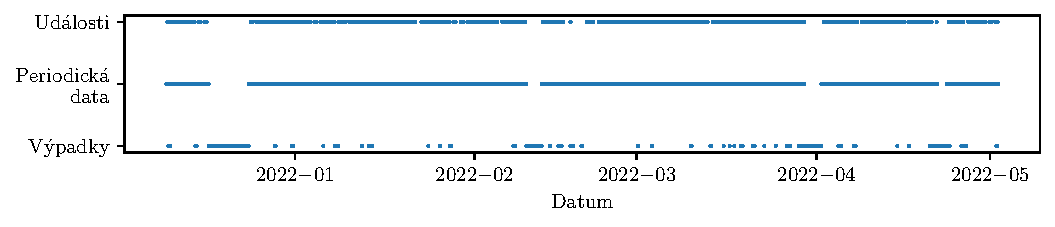
\includegraphics[draft=false,width=\textwidth]{img/results/sample_type.pdf}
        \caption[Graf druhu sesbíraných vzorků a výpadků]{Graf druhu sesbíraných vzorků dat a výpadků.}
        \label{fig:sample_type}
    \end{figure}
\section{Volba struktury \acrshort{nn} a parametrů učení}
    Na datech sesbíraných ve dnech od \DTMdisplaydate{2021}{12}{1}{-1} do \DTMdisplaydate{2022}{3}{17}{-1} bylo natrénováno 60 dopředných \acrshort{nn} (regresor FFNN, \cref{sec:ffnn}) a 32 rekurentních \acrshort{nn} (regresor LSTM, \cref{sec:lstm}). Dále budeme uvažovat pouze sítě trénované se ztrátovou funkcí \acrshort{mse}, protože ostatní se trénovaly s využitím kosinové vzdálenosti, která je pro danou úlohu nevhodná (nízkou ztrátu totiž vykazují nejen stavy blízko požadovaným, ale také ty, které mají blízký poměr mezi dvěma stavovými veličinami žaluzie), což se potvrdilo i při tomto experimentu, kdy \acrshort{mse} predikcí na testovací datové sadě (\cref{ssec:test}) u sítí trénovaných se ztrátovou funkcí \acrshort{mse} a s kosinovou podobností se lišila o řád jak v případě dopředné, tak i v případě rekurentní \acrshort{nn}. Struktura sítě, parametry použité při jejím trénování a \acrshort{mse} na testovací datové sadě jsou v \refskl{tab:ffnnhyperResults,tab:lstmhyperResults}{tabulkách}.
    % Table generated by Excel2LaTeX from sheet 'List1'
\begin{table}[htbp]
  \centering
  {
  \begin{tabular}{r|l|r|r|r}
    \toprule
          & Struktura & \multicolumn{1}{l|}{E} & \multicolumn{1}{l|}{BS} & \multicolumn{1}{l}{MSE} \\
    \midrule
    \midrule
    1     &  {[20, 15, 10]} & 500   & 32    & 0,01571 \\
    \midrule
    2     &  {[20, 15, 10]} & 700   & 32    & 0,01615 \\
    \midrule
    3     &  {[20, 15, 10]} & 500   & 16    & 0,01661 \\
    \midrule
    4     &  {[20, 15, 10]} & 200   & 32    & 0,01867 \\
    \midrule
    5     &  {[10, 15, 10]} & 700   & 16    & 0,01875 \\
    \midrule
    6     &  {[10, 15, 20]} & 700   & 16    & 0,01947 \\
    \midrule
    7     &  {[10, 15, 10]} & 500   & 16    & 0,01955 \\
    \midrule
    8     &  {[10, 15, 20]} & 500   & 32    & 0,02004 \\
    \midrule
    9     &  {[15, 10]} & 700   & 32    & 0,02071 \\
    \midrule
    10    &  {[20, 15, 10]} & 700   & 16    & 0,02119 \\
    \midrule
    11    &  {[15, 10]} & 700   & 16    & 0,02152 \\
    \midrule
    12    &  {[10, 15, 20]} & 500   & 16    & 0,02155 \\
    \midrule
    13    &  {[10, 15, 20]} & 200   & 16    & 0,02213 \\
    \midrule
    14    &  {[15, 10]} & 500   & 16    & 0,02214 \\
    \midrule
    15    &  {[10, 15, 10]} & 700   & 32    & 0,02297 \\
      \midrule
      16    &  {[10, 15, 10]} & 500   & 32    & 0,02451 \\
      \midrule
      17    &  {[10, 15, 20]} & 700   & 32    & 0,02478 \\
      \midrule
      18    &  {[20, 15, 10]} & 200   & 16    & 0,02543 \\
      \midrule
      19    &  {[10, 15]} & 700   & 32    & 0,02746 \\
      \midrule
      20    &  {[15, 10]} & 200   & 16    & 0,02752 \\
      \midrule
      21    &  {[10, 15, 10]} & 200   & 16    & 0,02914 \\
      \midrule
      22    &  {[10, 15]} & 700   & 16    & 0,02925 \\
      \midrule
      23    &  {[15, 10]} & 500   & 32    & 0,03059 \\
      \midrule
      24    &  {[10, 15]} & 200   & 16    & 0,03144 \\
      \midrule
      25    &  {[10, 15]} & 500   & 32    & 0,03357 \\
      \midrule
      26    &  {[10, 15]} & 200   & 32    & 0,04301 \\
      \midrule
      27    &  {[10, 15]} & 500   & 16    & 0,04732 \\
      \midrule
      28    &  {[10, 15, 20]} & 200   & 32    & 0,05163 \\
      \midrule
      29    &  {[15, 10]} & 200   & 32    & 0,05230 \\
      \midrule
      30    &  {[10, 15, 10]} & 200   & 32    & 0,05512 \\
      \bottomrule
      \bottomrule
      \end{tabular}%
      }
    \caption[Výsledky prohledávání parametrů FFNN]{Výsledky prohledávání parametrů dopředné neuronové sítě a jejího učení pro použití v systému automatického ovládání žaluzií. Sloupce: Struktura sítě, E - počet epoch trénování, BS - velikost dávky (batch size), MSE - střední kvadratická odchylka na testovací datové sadě.}
    \label{tab:ffnnhyperResults}%
\end{table}%

    % Table generated by Excel2LaTeX from sheet 'List1'
\begin{table}[htbp]
  \centering
    \begin{tabular}{r|l|r|r|r}
    \toprule
          & Struktura & \multicolumn{1}{l|}{E} & \multicolumn{1}{l|}{BS} & \multicolumn{1}{l}{MSE} \\
    \midrule
    \midrule
    1     & {[64, 64]} & 200   & 16    & 0,00348 \\
    \midrule
    2     & {[64, 32]} & 200   & 16    & 0,00357 \\
    \midrule
    3     & {[64, 16, 16]} & 200   & 16    & 0,00437 \\
    \midrule
    4     & {[64, 64]} & 200   & 64    & 0,00500 \\
    \midrule
    5     & {[64, 32]} & 100   & 16    & 0,00516 \\
    \midrule
    6     & {[64, 32]} & 200   & 64    & 0,00562 \\
    \midrule
    7     & {[64, 16]} & 200   & 16    & 0,00578 \\
    \midrule
    8     & {[64, 16]} & 200   & 64    & 0,00653 \\
    \midrule
    9     & {[64, 16, 16]} & 100   & 16    & 0,00657 \\
    \midrule
    10    & {[64, 16, 16]} & 200   & 64    & 0,00683 \\
    \midrule
    11    & {[64, 64]} & 100   & 16    & 0,00690 \\
    \midrule
    12    & {[64, 16]} & 100   & 64    & 0,00810 \\
    \midrule
    13    & {[64, 64]} & 100   & 64    & 0,00916 \\
    \midrule
    14    & {[64, 32]} & 100   & 64    & 0,00981 \\
    \midrule
    15    & {[64, 16]} & 100   & 16    & 0,00998 \\
    \midrule
    16    & {[64, 16, 16]} & 100   & 64    & 0,01058 \\
    \bottomrule
    \bottomrule
    \end{tabular}%
  \caption[Výsledky prohledávání parametrů LSTM]{Výsledky prohledávání parametrů rekurentní neuronové sítě a jejího učení pro použití v systému automatického ovládání žaluzií. Sloupce: Struktura sítě, E - počet epoch trénování, BS - velikost dávky (batch size), MSE - střední kvadratická odchylka na testovací datové sadě.}
  \label{tab:lstmhyperResults}%
\end{table}%


    Na základě těchto výsledků byly pro další použití v navrhovaném systému automatického ovládání žaluzií zvoleny následující parametry pro \acrshort{nn} a jejich trénování:
    \begin{itemize}
        \item Dopředná \acrshort{nn} (FFNN):
        \begin{itemize}
            \item 3 skryté vrstvy (po řadě 20, 15 a 10 neuronů);
            \item 500 epoch trénování;
            \item velikost dávky (batch\_size) 32.;
            \item ztrátová funkce (loss) \acrshort{mse}.
        \end{itemize}
        \item Dopředná \acrshort{nn} (LSTM):
        \begin{itemize}
            \item 2 skryté vrstvy (po řadě 64 a 64 neuronů);
            \item 200 epoch trénování;
            \item velikost dávky (batch\_size) 16;
            \item ztrátová funkce (loss) \acrshort{mse}.
        \end{itemize}
    \end{itemize}
\section{Vliv jednotlivých příznaků na predikci} \label{sec:res_features}
    Důležitost příznaků v regresorech byla vyjádřena jako průměrný rozdíl \acrshort{mse} jestliže jsou hodnoty daného příznaku náhodně promíchány mezi vzorky (20 realizací) a \acrshort{mse} na datech v původním pořadí. Pro regresor FFNN jsou první 4 nejdůležitější příznaky day\_secs, lum\_in, lum\_out a year\_day, pro regresor LSTM pak day\_secs, lum\_in, year\_day a owm\_wind\_speed. Mezi málo důležité příznaky patří u obou regresorů všechny teploty (temp\_in, temp\_out, owm\_temp\_$x$h pro $x=1,2,3$). Grafy důležitostí všech příznaků pro jednotlivé regresory jsou na \refskl{fig:pfi_ffnn,fig:pfi_lstm}{obrázcích}.
    \begin{figure}[H]
        \centering
        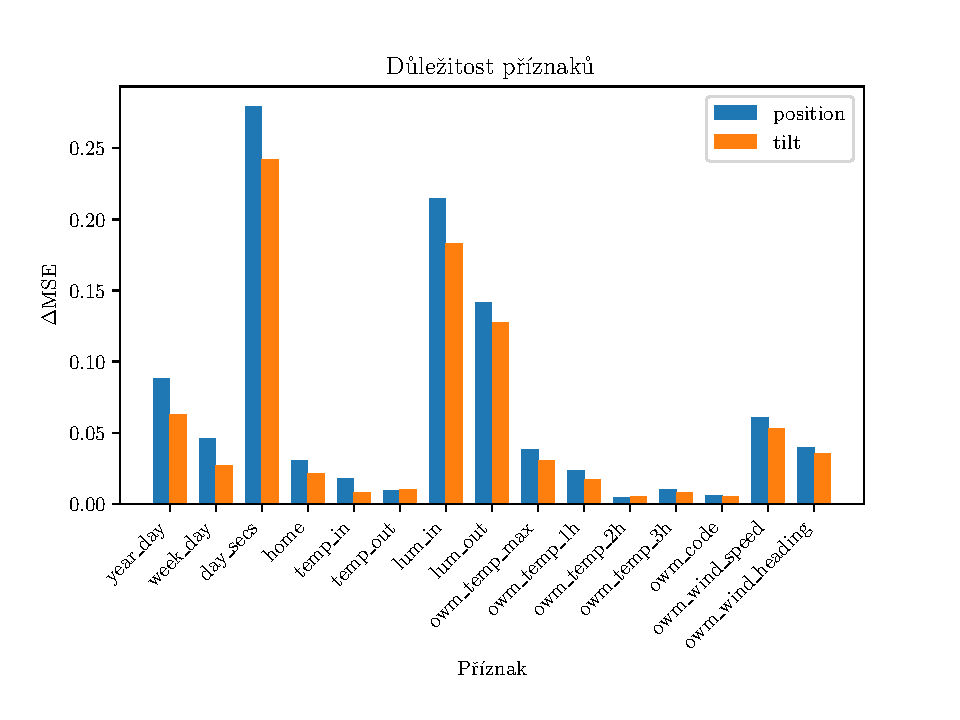
\includegraphics[draft=false,width=\textwidth]{img/results/pfi_ffnn.pdf}
        \caption[Důležitost příznaků FFNN]{Permutační důležilost příznaků v regresoru založeném na dopředné neuronové síti v úloze automatického ovládání žaluzie.}
        \label{fig:pfi_ffnn}
    \end{figure}
    \begin{figure}[H]
        \centering
        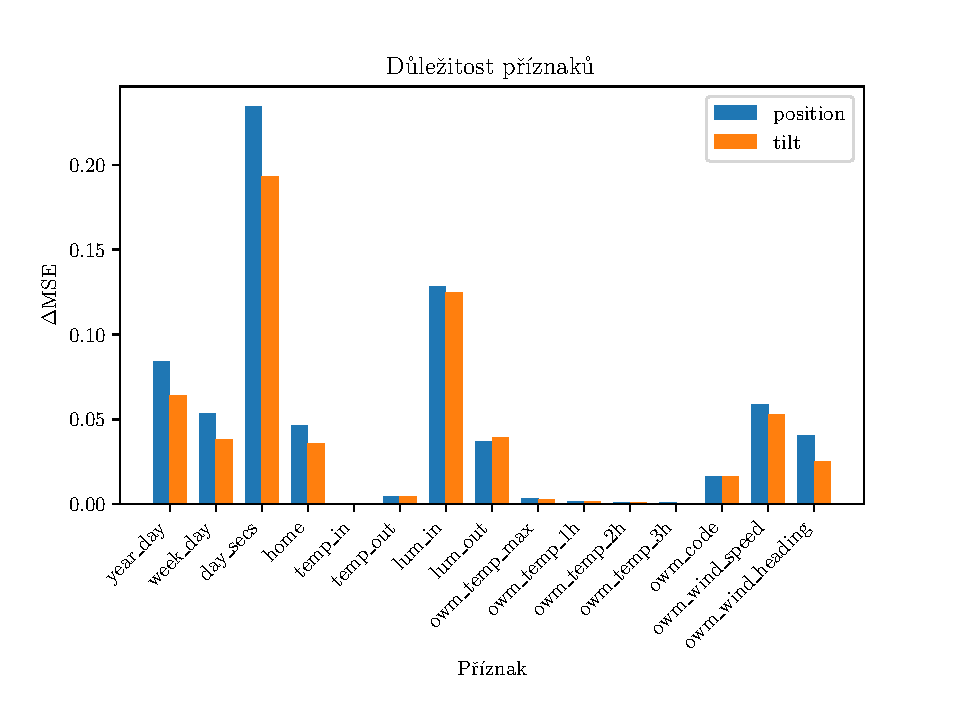
\includegraphics[draft=false,width=\textwidth]{img/results/pfi_lstm.pdf}
        \caption[Důležitost příznaků LSTM]{Permutační důležilost příznaků v regresoru založeném na rekurentní neuronové síti v úloze automatického ovládání žaluzie.}
        \label{fig:pfi_lstm}
    \end{figure}
\section{Porovnání regresorů} \label{sec:res_regr}
    Porovnání regresorů použitých v systému automatického ovládání žaluzie (jestliže to vzhledem k jejich návrhu dává smysl) z hlediska počtu parametrů (u Ifelse ručně konfigurované, u FFNN a LSTM odhadnuté pomocí algoritmů strojového učení), doby učení, doby predikce výstupu a dosažené \acrshort{mse} na testovací datové sadě je uvedené v \refskl{tab:regr_comp}{tabulce}. Regresor Ifelse má nejmenší počet parametrů, je 2. v rychlosti predikce a má nejvyšší \acrshort{mse}. Největší počet parametrů, dobu trénování i predikce a nejnižší \acrshort{mse} má regresor LSTM.
    % Table generated by Excel2LaTeX from sheet 'List1'
\begin{table}[htbp]
  \centering
    \begin{tabular}{l|r|r|r}
    \toprule
          & \multicolumn{1}{l|}{Ifelse} & \multicolumn{1}{l|}{FFNN} & \multicolumn{1}{l}{LSTM} \\
    \midrule
    \midrule
    Počet parametrů & 17    & 817   & 53634 \\
    \midrule
    Doba predikce [ms] & 250   & 30    & 430 \\
    \midrule
    Doba trénování [s] & -     & 1839  & 12129 \\
    \midrule
    MSE   & 0,120 & 0,0246 & 0,00426 \\
    \bottomrule
    \bottomrule
    \end{tabular}%
    \caption[Porovnání regresorů]{Porovnání vybraných vlastností regresorů. Doba predikce platí pro 400 vzorků.}
  \label{tab:regr_comp}%
\end{table}%


    Ukázka predikce obou stavových veličin žaluzie jednotlivými regresory na základě dat sesbíraných \DTMdisplaydate{2022}{04}{10}{-1} a porovnání se skutečným řízením je v grafu na \refskl{fig:regr_comp}{obrázku}.
    \begin{figure}[H]
        \centering
        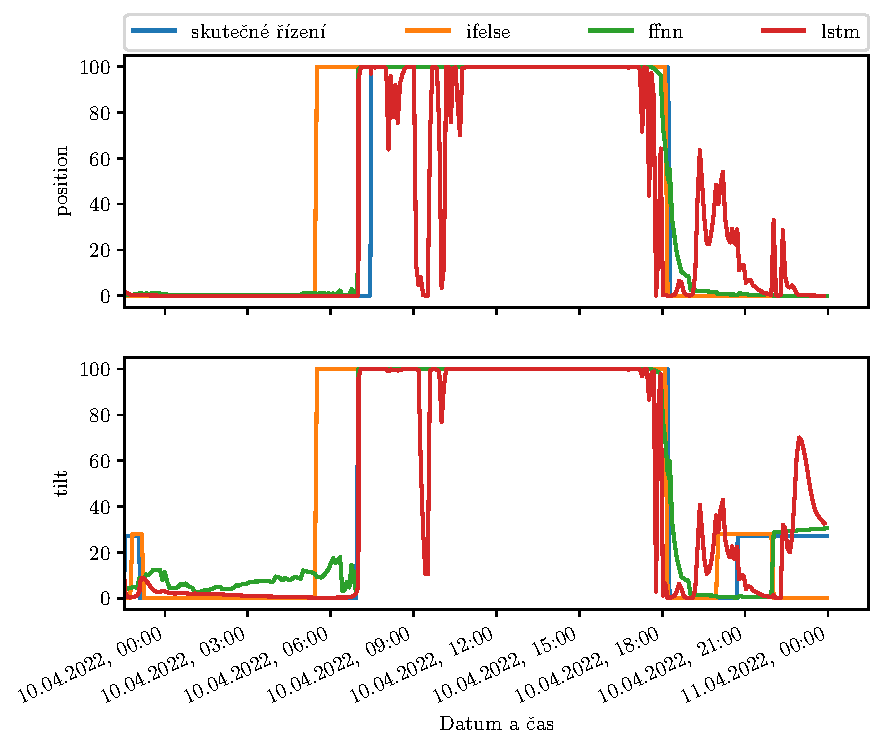
\includegraphics[draft=false,width=\textwidth]{img/results/regr_comp_sel.pdf}
        \caption[Porovnání predikce regresorů]{Porovnání predikce 3 regresorů a skutečného řízení na datech z \DTMdisplaydate{2022}{04}{10}{-1}}
        \label{fig:regr_comp}
    \end{figure}
\section{Vyhodnocení vlivu retrainingu} \label{sec:res_retr}
    Vyhodnocovat retraining má smysl jen u 2 z regresorů, které využívají strojové učení (FFNN a LSTM). Pro každý z nich se porovnaly 2 modely. První z modelů se trénovaly na datech do konce února, druhé pak vznikly z prvních opakovaným trénovaním na datech do konce dubna. \Cref{tab:retr_ffnn,tab:retr_lstm} porovnávají \acrshort{mse} od referenčních dat z testovací datové sady pro každý z regresorů celkově i pro každou stavovou proměnnou zvlášť.
    % Table generated by Excel2LaTeX from sheet 'retraining_ffnn'
\begin{table}[htbp]
  \centering
  \begin{tabular}{l|r|r|r}
    \toprule
          & \multicolumn{1}{l|}{celkově} & \multicolumn{1}{l|}{position} & \multicolumn{1}{l}{tilt} \\
    \midrule
    \midrule
    březen & 0,0962 & 0,1156 & 0,0769 \\
    \midrule
    květen & 0,0246 & 0,0329 & 0,0163 \\
    \bottomrule
    \bottomrule
    \end{tabular}%
  \caption[Retraining FFNN]{Porovnání středních kvadratických odchylek dvou modelů dopředné neuronové sítě natrénovaných na 2 různých datových sadách z období před daným měsícem.}
  \label{tab:retr_ffnn}%
\end{table}%

    % Table generated by Excel2LaTeX from sheet 'retraining_lstm'
\begin{table}[htbp]
  \centering
  \begin{tabular}{l|r|r|r}
  \toprule
        & \multicolumn{1}{l|}{celkově} & \multicolumn{1}{l|}{position} & \multicolumn{1}{l}{tilt} \\
  \midrule
  \midrule
  březen & 0,05911 & 0,07470 & 0,04351 \\
  \midrule
  květen & 0,00426 & 0,00316 & 0,00536 \\
  \bottomrule
  \bottomrule
  \end{tabular}%
    \caption[Retraining LSTM]{Porovnání středních kvadratických odchylek dvou modelů rekurentní neuronové sítě natrénovaných na 2 různých datových sadách z období před daným měsícem.}
    \label{tab:retr_lstm}%
\end{table}%


    Příklad predikce ovládání žaluzií (pro každou z proměnných ve vlastní soustavě souřadné) jednotlivými modely dne \DTMdisplaydate{2022}{04}{20}{-1} je na \refskl{fig:retr_ffnn,fig:retr_lstm}{obrázcích}.
    \begin{figure}[H]
        \centering
        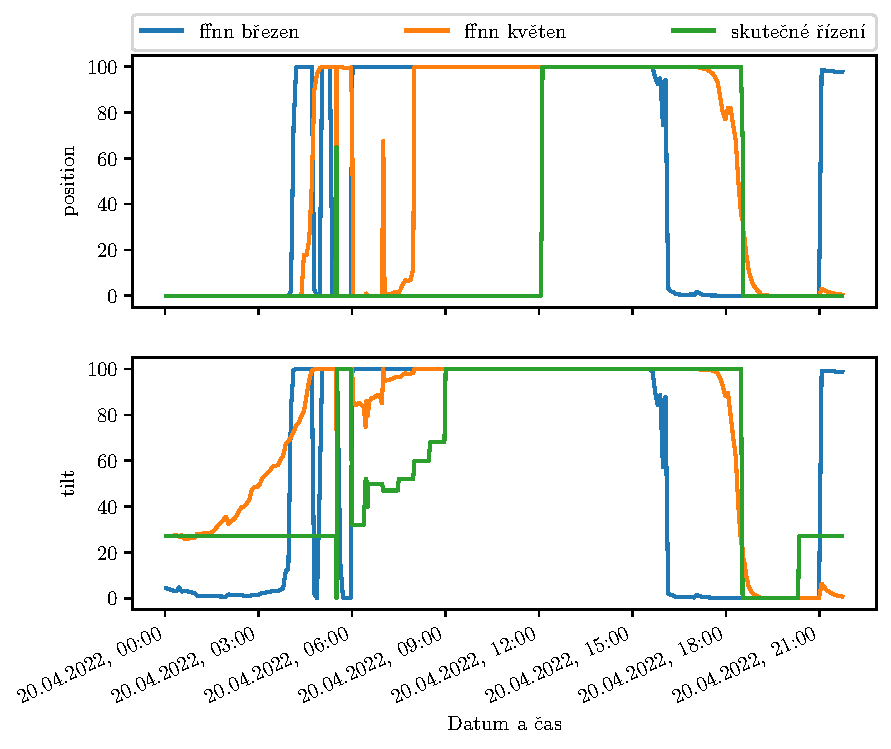
\includegraphics[draft=false,width=0.95\textwidth]{img/results/retraining_sel_ffnn.pdf}
        \caption[Porovnání predikce FFNN (retraining)]{Porovnání predikce 2 modelů dopředné neuronové sítě a skutečného řízení na datech z \DTMdisplaydate{2022}{04}{20}{-1}}
        \label{fig:retr_ffnn}
    \end{figure}
    \begin{figure}[H]
        \centering
        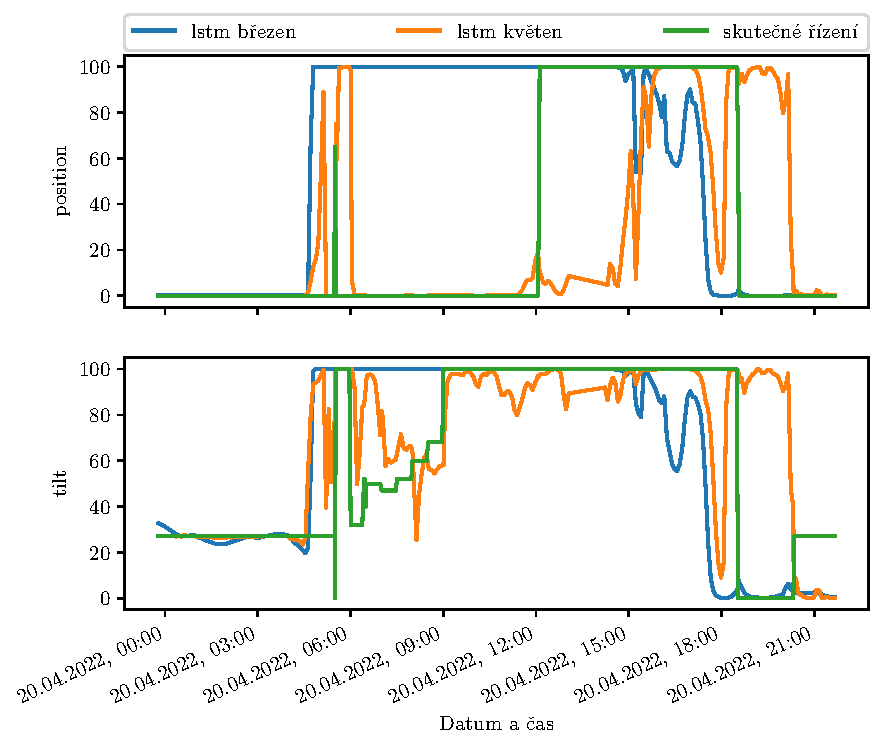
\includegraphics[draft=false,width=0.95\textwidth]{img/results/retraining_sel_lstm.pdf}
        \caption[Porovnání predikce LSTM (retraining)]{Porovnání predikce 2 modelů rekurentní neuronové sítě a skutečného řízení na datech z \DTMdisplaydate{2022}{04}{20}{-1}}
        \label{fig:retr_lstm}
    \end{figure}